\section{Определение ОРП с ошибками}
%\marginnote{\Date{Чт.}{12}{Июл.}{2018}}[-40pt]
\begin{itemize}

	\item Открываем 1С Розница 
	\item Переходим в журнал документов <<Отчеты о розничных продажах>> -
	\par
	\menu[,]{Продажи, Отчеты о розничных продажах, }
%	Сохраняем изменения \keys{ОК}
	 (Рис.~\ref{ris:1.jpg})	
	\begin{figure}[H]
		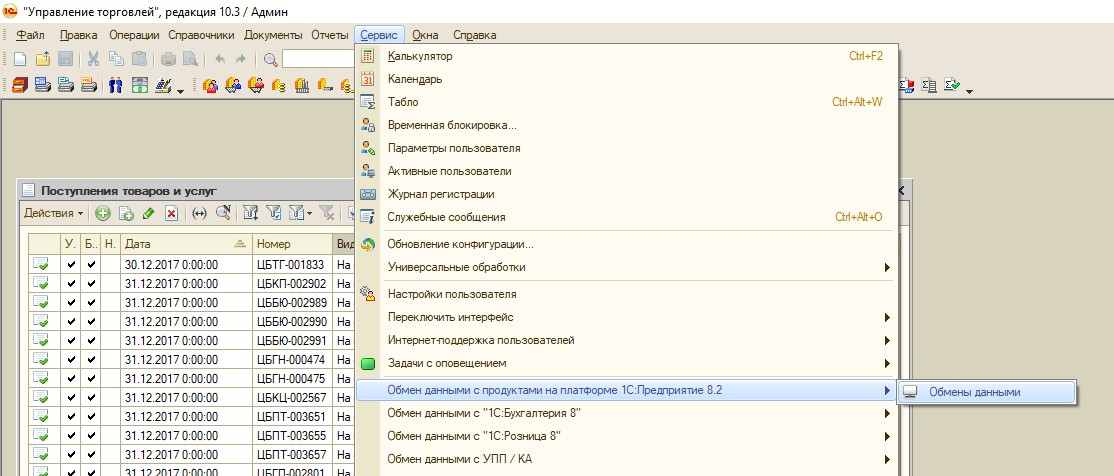
\includegraphics[width=0.8\textwidth]{1.jpg}
		\caption{журнал <<Отчеты о розничных продажах>>}
		\label{ris:1.jpg}
	\end{figure}
%	\item Наличие в журнале непроведенных документов, говорит о ошибках при закрытии кассовой смены.
	\item Находим первый не проведенный  ОРП.
	(Рис.~\ref{ris:2.jpg})	
	\begin{figure}[H]
		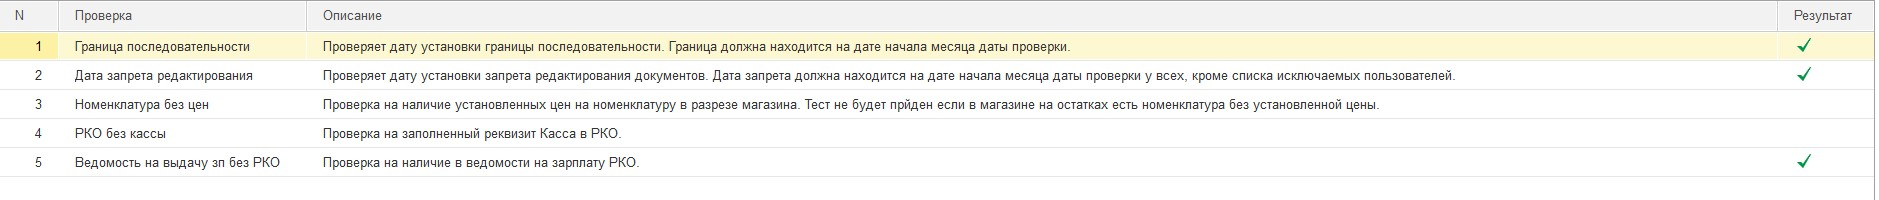
\includegraphics[width=0.7\textwidth]{2.jpg}
		\caption{Не проведенные документы.}
		\label{ris:2.jpg}
	\end{figure}
	
\newpage	
	\item Переходим на  вкладку <<Дополнительно>>.
	(Рис.~\ref{ris:3.jpg})	
	\begin{figure}[!ht]
		
		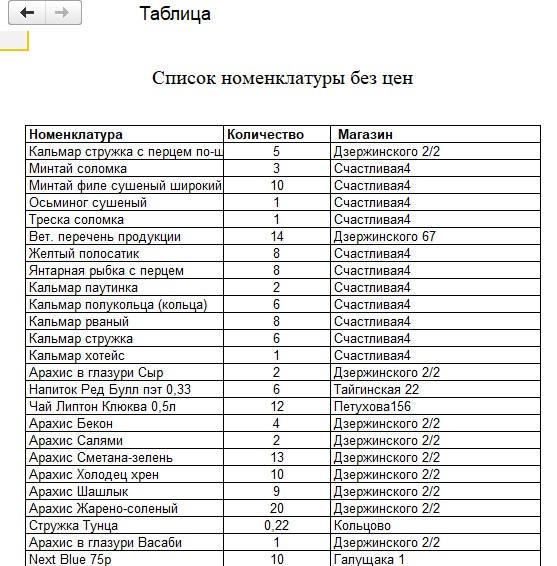
\includegraphics[width=1.0\textwidth]{3.jpg}
		\caption{Вкладка <<Дополнительно>>}
		\label{ris:3.jpg}
	\end{figure}

	\item На закладке <<Дополнительно>>,  в табличной части присутствует запись занесенная кассирами при закрытии смены.
	Если  в строке , в колонке «Брак»  галочка ОТСУТСТВУЕТ (Рис.~\ref{ris:4.jpg})
	то просто проводим ОРП. Если ОРП провелся то поиск ошибок в данном ОРП завершен.  После этого необходимо так же провести и отправить в ЕГАИС ,связанный с этим документом,  документ «Акт списания ЕГАИС» .\par
		
	\begin{figure}[!ht]
%		\fbox{Test figure 1}
		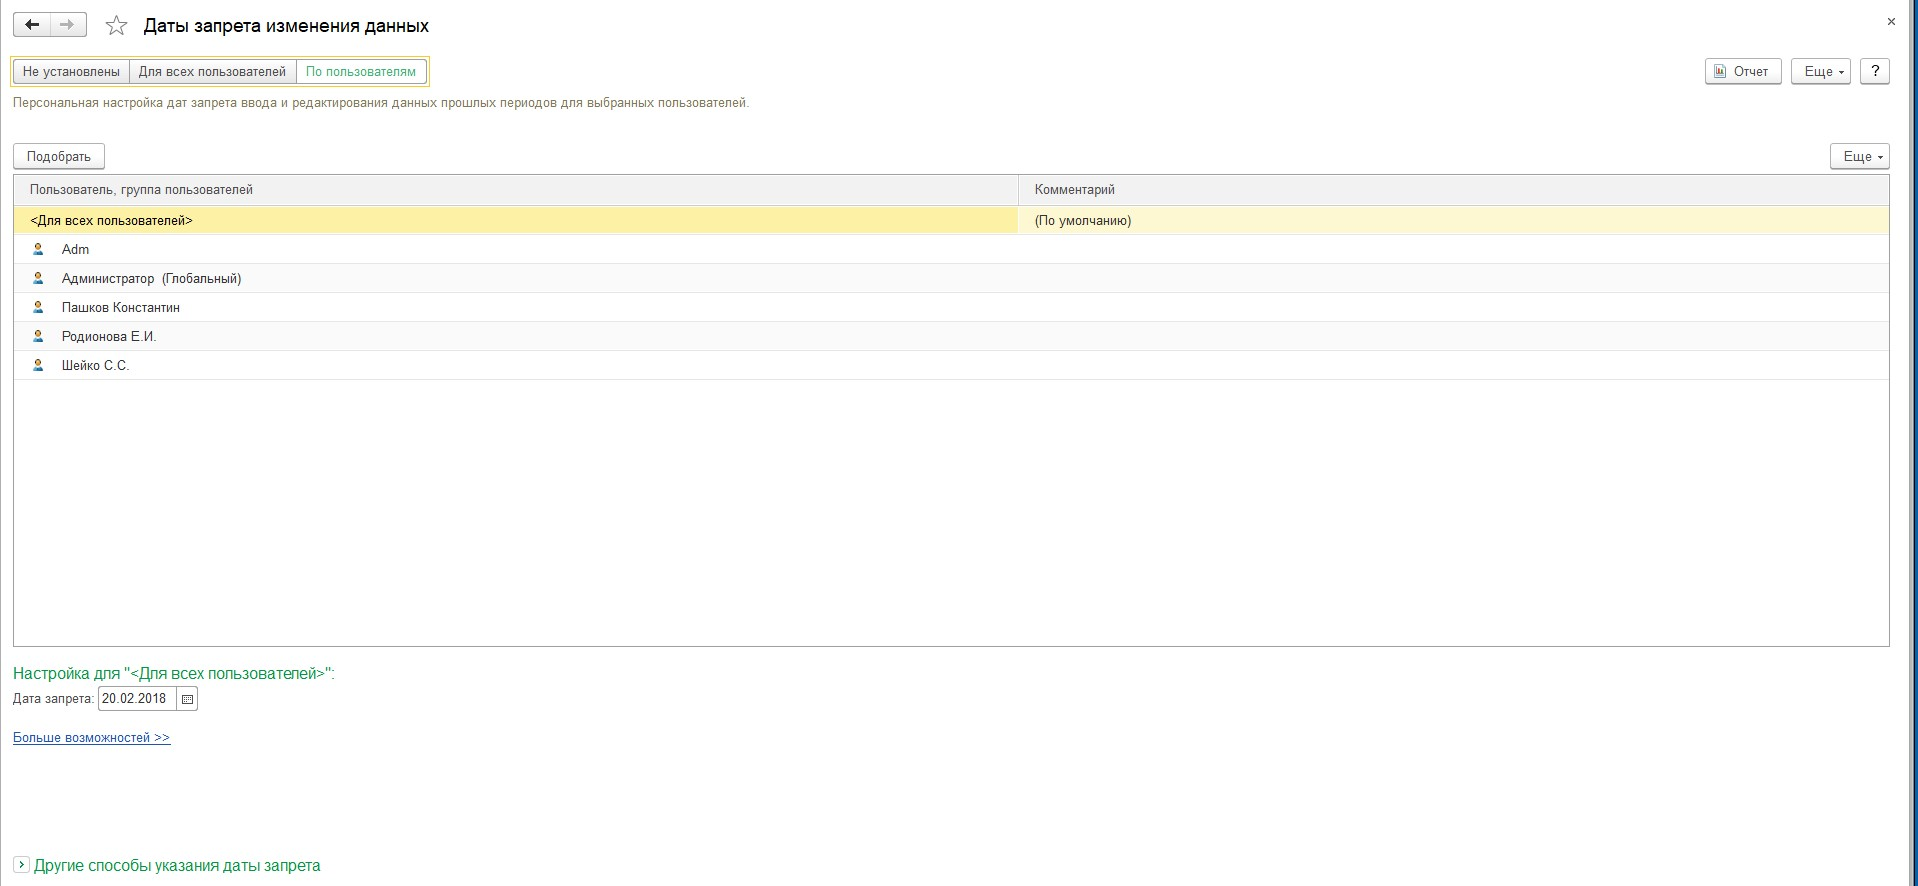
\includegraphics[width=0.35\textwidth]{4.jpg}
		\caption{Ошибки}
		\label{ris:4.jpg}
	\end{figure}

	\item Если в строке, в колонке «Брак»  галочка УСТАНОВЛЕНА (Рис. 1.4) то выполняем следующую последовательность действий:

	\begin{enumerate}[label={\alph*)},font={\color{red!50!black}\bfseries}] \label{100}
			\item Проверить правильность ввода данных кассирами при закрытии смены в соответствии с п.1 «Инструкции для кассиров». Для исправления этих ошибок дважды кликаем мышкой на строке с ошибками. Появляется окно редактирования (Рис.~\ref{ris:8.jpg}) \label{100}	
			
		\begin{figure}[H]
			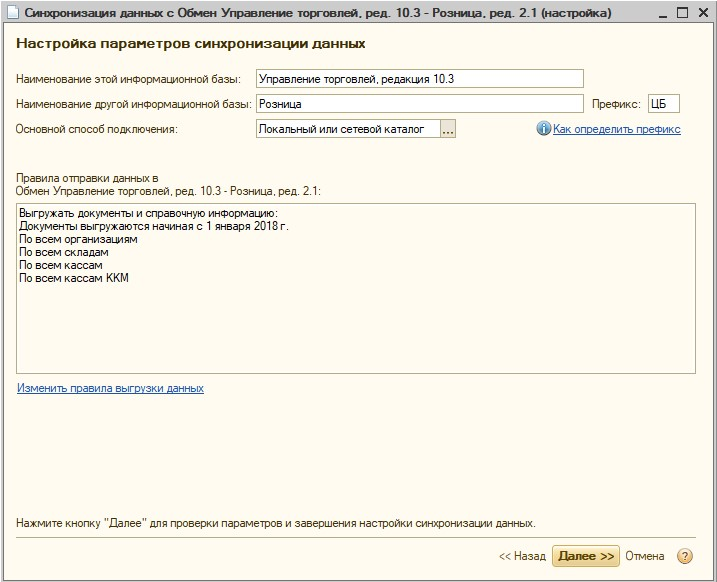
\includegraphics[width=0.4\textwidth]{8.jpg}
			\caption{Окно редактирования.}
			\label{ris:8.jpg}
		\end{figure}
			Сверяясь с бумажными документами заносим суммы в соответствующие поля. По окончании нажимаем \keys{Записать и закрыть}.
			Появляется новая строка с исправленными данными. Пробуем провести документ  ОРП. Если данные корректны, то документ поведется.
			Через меню <<Связанные документы>> (Рис.~\ref{ris:9.jpg})  переходим к <<Акту списания ЕГАИС>>.
		\begin{figure}[H]
			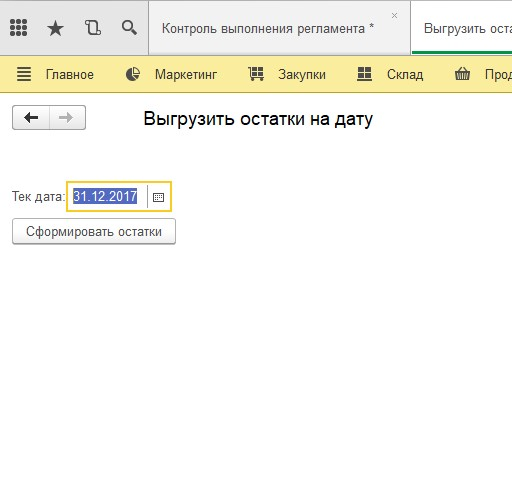
\includegraphics[width=0.6\textwidth]{9.jpg}
			\caption{Связанные документы.}
			\label{ris:9.jpg}
		\end{figure}
	 	\begin{figure}[H]
			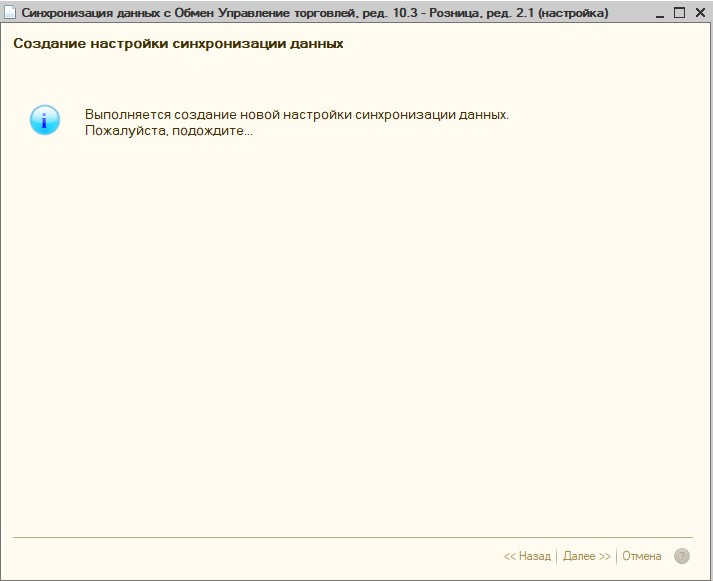
\includegraphics[width=0.9\textwidth]{10.jpg}
			\caption{Акт списания ЕГАИС.}
			\label{ris:10.jpg}
		\end{figure}
			Проводим его и отправляем в ЕГАИС. (Рис.~\ref{ris:10.jpg})
			Если ОРП провелся то поиск ошибок в данном ОРП завершен. 
		\item Если после выполнения проверки изложенной в п. \ref{100}   документ ОРП не провелся переходим к поиску ошибок в соответствии с методикой описанной в п. \ref{5000} настоящего руководства. 
	\end{enumerate}
	
\end{itemize}
